\section{问题四：干基质量坐标下的收缩动边界干燥模型}\label{sec:p4}

\subsection{相对问题三的增量：从固定域到移动边界}

问题四在问题三的时变边界基础上，进一步计入附件2 观测到的体积收缩：干燥过程中半径由
$R_0=2\,\mathrm{cm}$ 单调缩小，变物性改用附录4，即在式~\eqref{eq:diff} 的 Arrhenius 扩散律中取
前因子 $D_0=4.2\times10^{-4}$、浓度指数 $a=0.30$、活化温标 $E=3850\,\mathrm{K}$，其余密度、比热与
导热率随含水率 $C$（干基，kg 水/kg 干物质）线性/饱和变化：
\begin{equation}\label{eq:p4props}
\begin{aligned}
\rho(C)&=760+90C, & c_p(C)&=1850+2150\frac{C}{C+1},\\
k(C)&=0.12+0.20\frac{C}{C+1}, & D(C,T)&=4.2\times10^{-4}\,e^{-0.30/C}\,e^{-3850/T_K},
\end{aligned}
\end{equation}
式~\eqref{eq:p4props} 中 $T_K=T+273.15$ 为开尔文温度，$\rho$（$\mathrm{kg/m^3}$）、$c_p$
（$\mathrm{J/(kg\,K)}$）、$k$（$\mathrm{W/(m\,K)}$）、$D$（$\mathrm{m^2/s}$）均为 $C$（及 $T$）的函数，
与问题三附录3 相比前因子降低约一个数量级、浓度指数由 $0.89$ 降为 $0.30$，故同一含水率下附录4
扩散更弱、温度敏感度相当。附件2 半径数据经 PCHIP 单调插值得到 $R(t)$，见图~\ref{fig:radius_shrink}。

\begin{figure}[H]
  \centering
  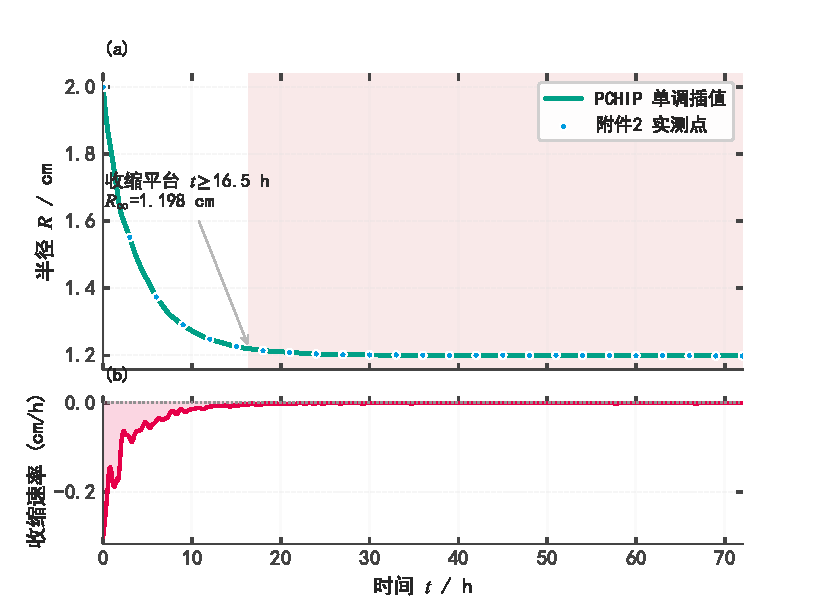
\includegraphics[width=0.9\textwidth,height=0.8\textheight,keepaspectratio]{../figures/fig_radius_shrink.pdf}
  \caption{附件2 半径收缩数据的 PCHIP 单调插值曲线与收缩速率}
  \label{fig:radius_shrink}
\end{figure}

图~\ref{fig:radius_shrink} 采用 PCHIP（分段三次 Hermite 保单调插值）而非普通三次样条，以
避免样条过冲产生半径回升的非物理现象；插值在数据节点处精确复现（表~\ref{tab:verification}
中 PCHIP 复现误差为 $0$）。收缩使求解域随时间变化，直接在 $r$ 上离散会遭遇动网格困难，
故引入固定域映射。

\subsection{Landau 固定域映射与干基质量不变量}

令 $\xi=r/R(t)\in[0,1]$，把随时间收缩的物理域 $[0,R(t)]$ 映射到固定域 $[0,1]$，映射关系见
图~\ref{fig:tikz_landau_map}。

\begin{figure}[H]
  \centering
  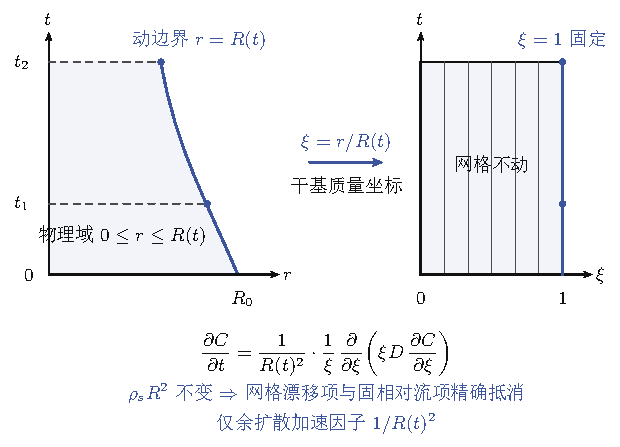
\includegraphics[width=0.9\textwidth,height=0.8\textheight,keepaspectratio]{../figures/tikz_landau_map.pdf}
  \caption{收缩物理域 $[0,R(t)]$ 到固定计算域 $[0,1]$ 的 Landau 坐标映射}
  \label{fig:tikz_landau_map}
\end{figure}

收缩使干骨架随物质点内移，$\rho_s$ 不再是常数、不能从水分方程两侧约去，故须保留 $\rho_s$ 写出物理域
$[0,R(t)]$ 上的干物质基守恒型水分方程
\begin{equation}\label{eq:p4phys}
\left.\frac{\partial}{\partial t}\big(\rho_s C\big)\right|_{r}
+\frac1r\frac{\partial}{\partial r}\big(r\,\rho_s C\,v_s\big)
=\frac1r\frac{\partial}{\partial r}\!\left(r\,\rho_s D\frac{\partial C}{\partial r}\right),
\end{equation}
其中 $v_s$ 为固相基质径向速度；由 $r=\xi R(t)$ 且物质点 $\xi$ 不变，得 $v_s=\xi\dot R$。固定 $\xi$ 与固定 $r$
求时间导数、以及径向导数之间的坐标变换算子恒等式为
\begin{equation}\label{eq:p4map}
\left.\frac{\partial}{\partial t}\right|_{r}
=\left.\frac{\partial}{\partial t}\right|_{\xi}-\frac{\dot R}{R}\,\xi\,\frac{\partial}{\partial\xi},
\qquad
\frac{\partial}{\partial r}=\frac1R\frac{\partial}{\partial\xi}.
\end{equation}
式~\eqref{eq:p4map} 左式的第二项即随域收缩产生的\textbf{映射漂移（伪对流）项}。关键化简来自
\textbf{干物质总量守恒}：由假设 H6（干骨架不滑移），单位长度圆柱内 $[0,\xi]$ 的干物质量
$\pi\rho_s R^2\xi^2$ 对任意 $\xi$ 守恒，对时间求导得纯径向收缩下的不变量
\begin{equation}\label{eq:drymass}
\rho_s(t)\,R(t)^2=\sigma=\mathrm{const},
\end{equation}
即式~\eqref{eq:drymass} 表明 $\rho_s$ 与 $R^2$ 反比变化，等价地 $\dot\rho_s/\rho_s=-2\dot R/R$。以此为支点，把式~\eqref{eq:p4map}
代入式~\eqref{eq:p4phys}：$v_s=\xi\dot R$ 引入的映射漂移项 $-\rho_s\frac{\xi\dot R}{R}\partial_\xi C$
与固相对流项 $+\rho_s\frac{\xi\dot R}{R}\partial_\xi C$ 恰好\textbf{两两抵消}，其余 $C$ 系数项借
$\dot\rho_s/\rho_s=-2\dot R/R$ 成对消去，两侧再同除只依赖 $t$ 的 $\rho_s$，使含水率方程在固定域上收敛为单一的
$1/R(t)^2$ 因子形式（推导见图~\ref{fig:tikz_drymass_derive}）：
\begin{equation}\label{eq:landau}
\left.\frac{\partial C}{\partial t}\right|_{\xi}
=\frac{1}{R(t)^2}\,\frac{1}{\xi}\frac{\partial}{\partial\xi}\!\left(\xi\,D\,\frac{\partial C}{\partial\xi}\right),
\qquad \xi\in(0,1) .
\end{equation}

\begin{figure}[H]
  \centering
  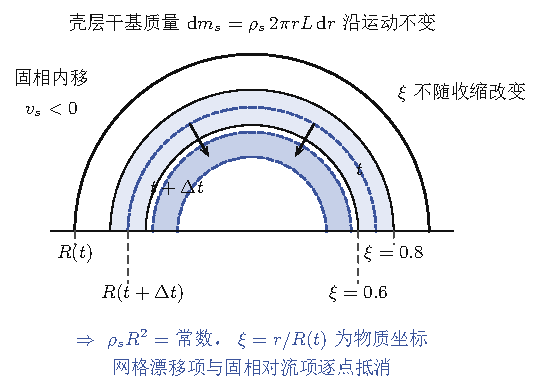
\includegraphics[width=0.9\textwidth,height=0.8\textheight,keepaspectratio]{../figures/tikz_drymass_derive.pdf}
  \caption{干基质量不变量 $\rho_s R^2=\sigma$ 导致收缩对流项与度规项两项抵消}
  \label{fig:tikz_drymass_derive}
\end{figure}

图~\ref{fig:tikz_drymass_derive} 展示了两项抵消的代数结构：正是干物质守恒把看似复杂的动边界
对流—扩散问题化简为固定域上仅含时变系数 $1/R(t)^2$ 的扩散方程，从而可直接沿用公共内核的
有限体积离散式~\eqref{eq:fvm}、界面 Kirchhoff 积分平均式~\eqref{eq:kirchhoff} 与后向 Euler/Picard
推进式~\eqref{eq:picard}，只需把式~\eqref{eq:fvm} 中的扩散通量整体乘以当前的 $1/R(t)^2$ 因子。式~\eqref{eq:landau}
把移动边界的全部几何效应\textbf{凝聚为单一时变因子}，是本问建模的核心。温度方程在同一映射下作
完全同构的变换，得固定域上的能量方程
\begin{equation}\label{eq:landauT}
\rho c_p\left.\frac{\partial T}{\partial t}\right|_{\xi}
=\frac{1}{R(t)^2}\,\frac1\xi\frac{\partial}{\partial\xi}\!\left(\xi\,k\,\frac{\partial T}{\partial\xi}\right),
\qquad \xi\in(0,1).
\end{equation}
式~\eqref{eq:landauT} 与式~\eqref{eq:landau} 共享同一 $1/R(t)^2$ 收缩因子，温度与含水率经变物性
$\rho(C)$、$c_p(C)$、$k(C)$、$D(C,T)$ 在同一 Picard 回路内双向耦合求解。

固定域上的边界条件相应改写：中心 $\xi=0$ 处由对称性得 $\partial_\xi C|_{\xi=0}=\partial_\xi T|_{\xi=0}=0$；
表面 $\xi=1$ 处因物理梯度 $\partial_r C=\frac1R\partial_\xi C$，Robin 传质/传热条件变为
\begin{equation}\label{eq:p4bc}
-\frac{D}{R(t)}\frac{\partial C}{\partial\xi}\bigg|_{\xi=1}=h_m\big(C_s-C_{air}\big),
\qquad
-\frac{k}{R(t)}\frac{\partial T}{\partial\xi}\bigg|_{\xi=1}=h\big(T_s-T_{air}\big).
\end{equation}
式~\eqref{eq:p4bc} 中 $R(t)$ 进入边界条件：随半径收缩，同一浓度差对应更陡的 $\xi$ 梯度。

定义干基质量加权平均含水率，其权重 $\xi$ 来自柱几何的面积测度
\begin{equation}\label{eq:cbar}
\bar C(t)=\frac{\int_0^1 C(\xi,t)\,\xi\,\mathrm{d}\xi}{\int_0^1 \xi\,\mathrm{d}\xi}
        =2\int_0^1 C(\xi,t)\,\xi\,\mathrm{d}\xi .
\end{equation}
对式~\eqref{eq:landau} 两侧乘 $2\xi$ 沿 $[0,1]$ 积分，中心项因面积为零而消失，表面项代入
式~\eqref{eq:p4bc}，即得关于式~\eqref{eq:cbar} 所定义 $\bar C(t)$ 的\textbf{精确整体平衡律}
\begin{equation}\label{eq:p4balance}
\frac{\mathrm{d}\bar C}{\mathrm{d}t}=-\frac{2h_m}{R(t)}\big(C_s-C_{air}\big).
\end{equation}
式~\eqref{eq:p4balance} 把二维时空场的正确性压缩为一个标量恒等式，是最有力的数值审计工具：实现层
逐步累加右端与左端实际变化比较，实测守恒残差落在 $5\times10^{-16}$–$4\times10^{-14}$（机器精度量级），
任何遗漏 $1/R^2$ 因子或错用界面平均的实现都会在此暴露为 $10^{-3}$ 以上的偏差（见第~\ref{sec:verify} 节）。

\subsection{收缩方式假设的独立数据检验}

式~\eqref{eq:landau} 依赖"纯径向均匀收缩、干物质守恒"这一假设。为避免循环论证，用附件2
自身数据独立检验收缩方式，见图~\ref{fig:shrink_evidence}。

\begin{figure}[H]
  \centering
  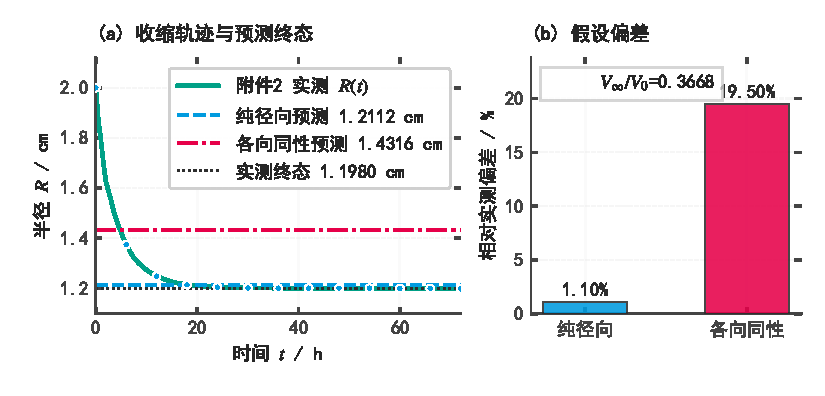
\includegraphics[width=0.9\textwidth,height=0.8\textheight,keepaspectratio]{../figures/fig_shrink_evidence.pdf}
  \caption{收缩方式假设的独立数据检验：观测终态体积比与各向同性/纯径向预测的对照}
  \label{fig:shrink_evidence}
\end{figure}

图~\ref{fig:shrink_evidence} 显示，附件2 的终态体积比 $V_\infty/V_0=0.3668$；若假设纯径向收缩
（长度不变），反推终态半径 $1.2112\,\mathrm{cm}$，与观测终值 $1.2\,\mathrm{cm}$ 仅差 $1.10\%$；
而若假设各向同性收缩（长度同比缩短），反推半径 $1.4316\,\mathrm{cm}$，偏差高达 $19.50\%$。
\textbf{纯径向假设与数据高度一致}，各向同性假设被数据否定，故式~\eqref{eq:landau} 的收缩方式
设定得到实测支持，而非任意选取。

\subsection{结果与问题三的正交分解比较}

图~\ref{fig:shrink_field} 给出收缩域内的含水率场与移动边界轨迹。

\begin{figure}[H]
  \centering
  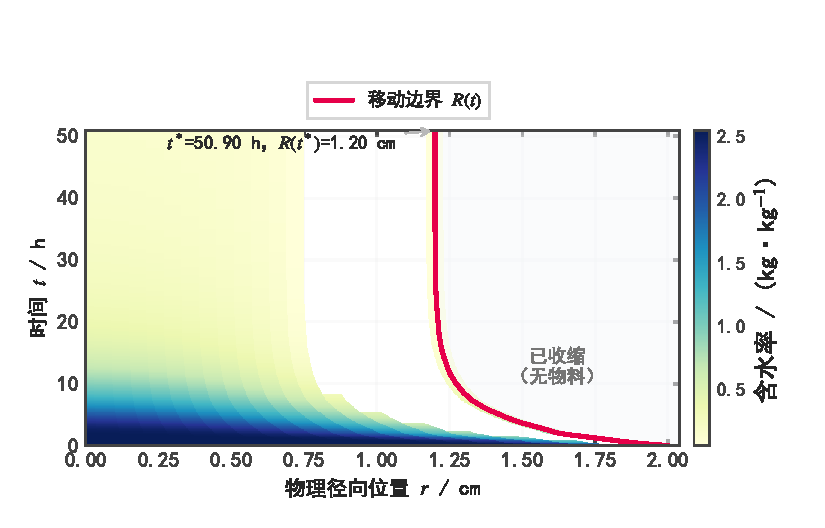
\includegraphics[width=0.9\textwidth,height=0.8\textheight,keepaspectratio]{../figures/fig_shrink_field.pdf}
  \caption{问题4 收缩域含水率场 $C(r,t)$ 与移动边界 $R(t)$ 的轨迹}
  \label{fig:shrink_field}
\end{figure}

由图~\ref{fig:shrink_field}，沿用式~\eqref{eq:endpoint} 的首次穿越判据（此处 $C(r,t)$ 在收缩域
$[0,R(t)]$ 上取，轴心仍为最慢点），计入收缩后达标时刻 $t^{*}=50.898\,\mathrm{h}$（此刻
$\max_r C=0.14999544$，前一步 $0.15003$），比问题三的 $57.262\,\mathrm{h}$ \textbf{缩短约 $11\%$}；
达标时半径已收缩到 $R(t^{*})=1.20\,\mathrm{cm}$。轴心含水率每 $6\,\mathrm{h}$ 依次为
$1.716,0.735,0.407,0.284,0.226,0.192,0.171,0.156$，同期半径为
$1.374,1.248,1.214,1.204,1.201,1.200,1.200,1.200\,\mathrm{cm}$，收缩主要发生在前 $12\,\mathrm{h}$、
随后趋稳。收缩缩短干燥期的原因有二：扩散路径变短、以及 $1/R^2$ 因子放大有效扩散。为把
这两种效应与"物性由附录3 换成附录4"的效应分离，作 $2\times2$ 正交分解，见
图~\ref{fig:orthogonal_waterfall}。

\begin{figure}[H]
  \centering
  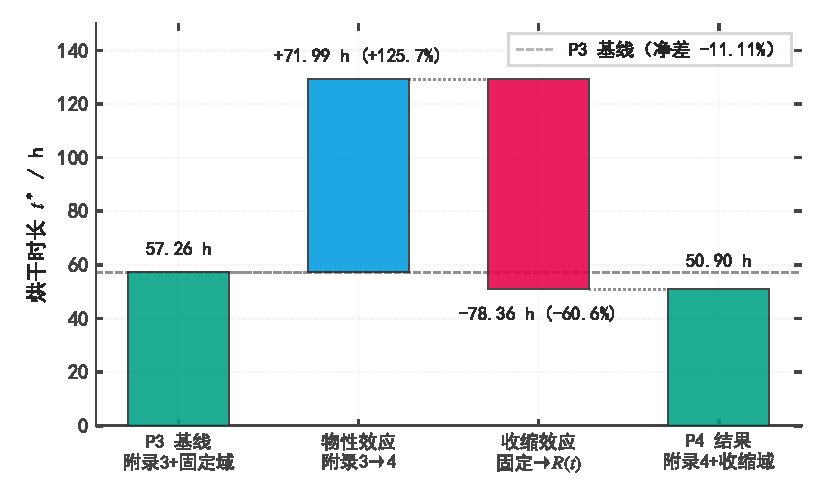
\includegraphics[width=0.9\textwidth,height=0.8\textheight,keepaspectratio]{../figures/fig_orthogonal_waterfall.pdf}
  \caption{问题4 与问题3 达标时刻差异的正交分解（物性效应与收缩效应）}
  \label{fig:orthogonal_waterfall}
\end{figure}

图~\ref{fig:orthogonal_waterfall} 通过瀑布图把 $57.262\to50.898\,\mathrm{h}$ 的变化拆为可加的
两部分：\textbf{收缩效应显著缩短干燥期，而附录3$\to$附录4 的物性变化方向相反}，二者部分抵消，
净效应为缩短约 $11\%$。这一分解说明"计入收缩使干燥更快"的结论对物性选择稳健，是收缩
几何本身的作用，而非附录切换的假象。若强行忽略收缩（问题4 退化为固定域），$t^*$ 将虚高到
$129.25\,\mathrm{h}$（见第\ref{sec:sens}节），进一步佐证动边界是本问不可省略的机制。各问结果汇总
见表~\ref{tab:main_results}。

% 表：四问核心结果汇总
% 数据来源：figures/all_results.json, problem_1..4_results.json, result1-4.xlsx
\begin{table}[H]
  \centering
  \caption{四问核心求解结果汇总}
  \label{tab:main_results}
  \small
  \begin{tabular}{clcrrrl}
    \toprule
    问题 & 物性/工况 & 时程 & 输出行数 & $C$ 中心终值 & $C$ 表面终值 & 达标时刻 $t^*$ \\
    \midrule
    1 & 附录2 常物性       & $0\sim1800$ s   & 1801  & 2.5500 & 1.5125 & 预热段，不反演 \\
    2 & 附录3 变物性       & $0\sim3$ h      & 10801 & 1.7662 & 1.0078 & 未达标 \\
    3 & 附录3 + 附件1 环境 & $0\sim57.26$ h  & 3437  & 0.1500 & 0.0525 & 57.262 h \\
    4 & 附录4 + 动边界     & $0\sim50.90$ h  & 3055  & 0.1500 & 0.0525 & 50.898 h \\
    \bottomrule
  \end{tabular}

  \vspace{2pt}
  \parbox{0.92\linewidth}{\footnotesize
  注：含水率为干基，单位 kg$\cdot$kg$^{-1}$；达标判据为全域最大含水率
  $\max_r C\le 0.15$。问题 1、2 时程由题面给定，终点含水率仍高于阈值，
  故不存在 $t^*$。问题 4 表面指动边界 $r=R(t)$ 处，$t^*$ 时刻 $R=1.2$ cm。}
\end{table}


